\section{Architectural Design}
\subsection{Overview}
The CodeKataBattles system is architecturally designed as a web-based application with a client-server architecture. The primary components include:
\begin{itemize}
    \item \textbf{Client interface}: A web-based user interface accessed by both students and educators. It provides the functionalities for participating in code katas (battles), joining tournaments, and viewing performance metrics (i.e. battle or tournament rankings).
    \item \textbf{Server Backend}: The backend serves as the brain of the system used to handle user requests, process and store data, and communicate with external services, such as GitHub. 
 
    \item \textbf{GitHub Integration}: The system leverages GitHub as a version control and repository hosting service. This integration is crucial for managing code submissions, automating code testing/evaluation, and ensuring version control.
\end{itemize}

The system shall be built as a distributed system with a three-tier architecture. It includes the topmost layer; the presentation tier (client tier), presenting information and user interface elements to users, the application tier (logic tier), containing the business logic that enables the systems core functionalities by communicating with the database and other external services to retrieve or update data, and the bottom layer; the data tier, dealing with the data storage, retrieval, and management (see fig. \ref{fig:3tierArchitecture}).


\begin{figure}[H]
    \centering
    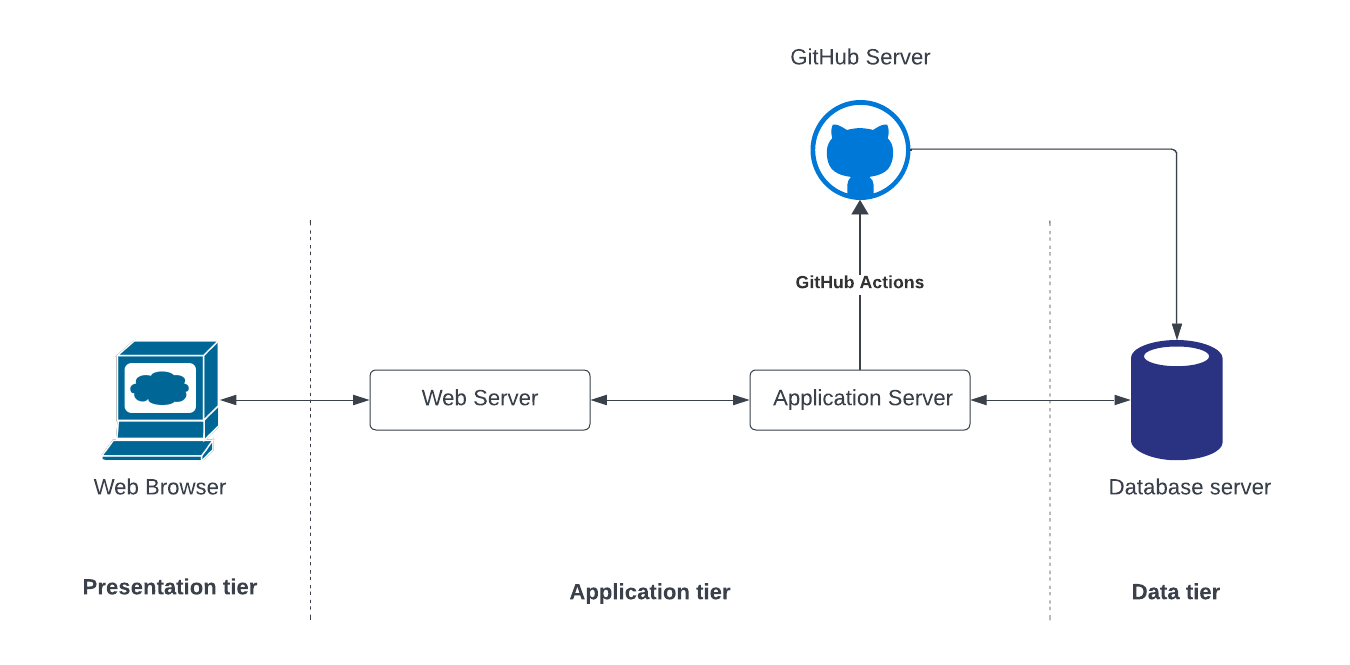
\includegraphics[width=\textwidth]{Graphics/Architecture/3-tier architecture.png}
    \caption{High level system architecture}
    \label{fig:3tierArchitecture}
\end{figure}

The external service integration most crucial to the CodeKataBattle's main functionality is the integration of GitHub. This is enabled through GitHub Actions which allows for the setting up of workflows that automate tasks based on events in specific GitHub repositories. This aspect falls under the system's Application Tier, which consists of the Webserver, the Application Server, and the communication with the Github Server. 

Regarding the internal set-up of the application tier, an event-driven architecture has been chosen, as this is greatly supported by GitHub Actions. The deployment of GitHub actions removes the necessity to build or integrate event brokers, publishers or subscribers, as this is handled by the action yaml-file (see fig. \ref{fig:EventFlow}). 

Every single Battle will simply consist of a standardised GitHub repository with standardised actions built in. The actions ensure that, upon a push to a forked repository, certain specified test files are run and the results are subsequently written to the database, if the push occurs within the battle time limit. 

The effective scaling of the testing modules in case of increased amount of submissions to a battle immediately before the deadline, has been identified as a potential bottleneck of the system. However, as GitHub Actions spins up an independent container for each event (e.g. a push) being handled, it harvests the strengths of a microservice architecture and averts this specific bottleneck.

The workload is split between three physical infrastructures; The submissions and testing occurs on GitHub’s infrastructure, The application is hosted on the application and web server, and the database containing the results are secluded on the database server (see fig. \ref{fig:physicalpartitions}). 
The Application Server "writes" to the GitHub server only to trigger the creation of a new battle repository upon educator input. In response GitHub actions provides the battle repository URL, which it writes to the database, from where the Application Server reads it. Thus the Application Server "writes" to the GitHub server and the Github server "writes" to the database (see fig. \ref{fig:3tierArchitecture}).

This physical dichotomy means that most of the workload is going to be placed on the container-based infrastructure of GitHub Actions, decreasing the requirements for the remaining infrastructure in order to remain scalable. The Web-server simply needs to support users reviewing their results and rankings of their battles, while all the scoring is handled in another system. While scoring of submissions are performed in relative parallel, potential bottlenecks can occur if many submissions are made at the same time, creating a long write-queue to the database, potentially increasing the time from a submission is made until the result is visible on the web app. Another potential bottleneck is simply that of many sign-ins and requests for battle results, for which we currently don't supply any mitigation strategy, as it is unclear how badly it will scale with user count.

\begin{figure}[H]
    \centering
    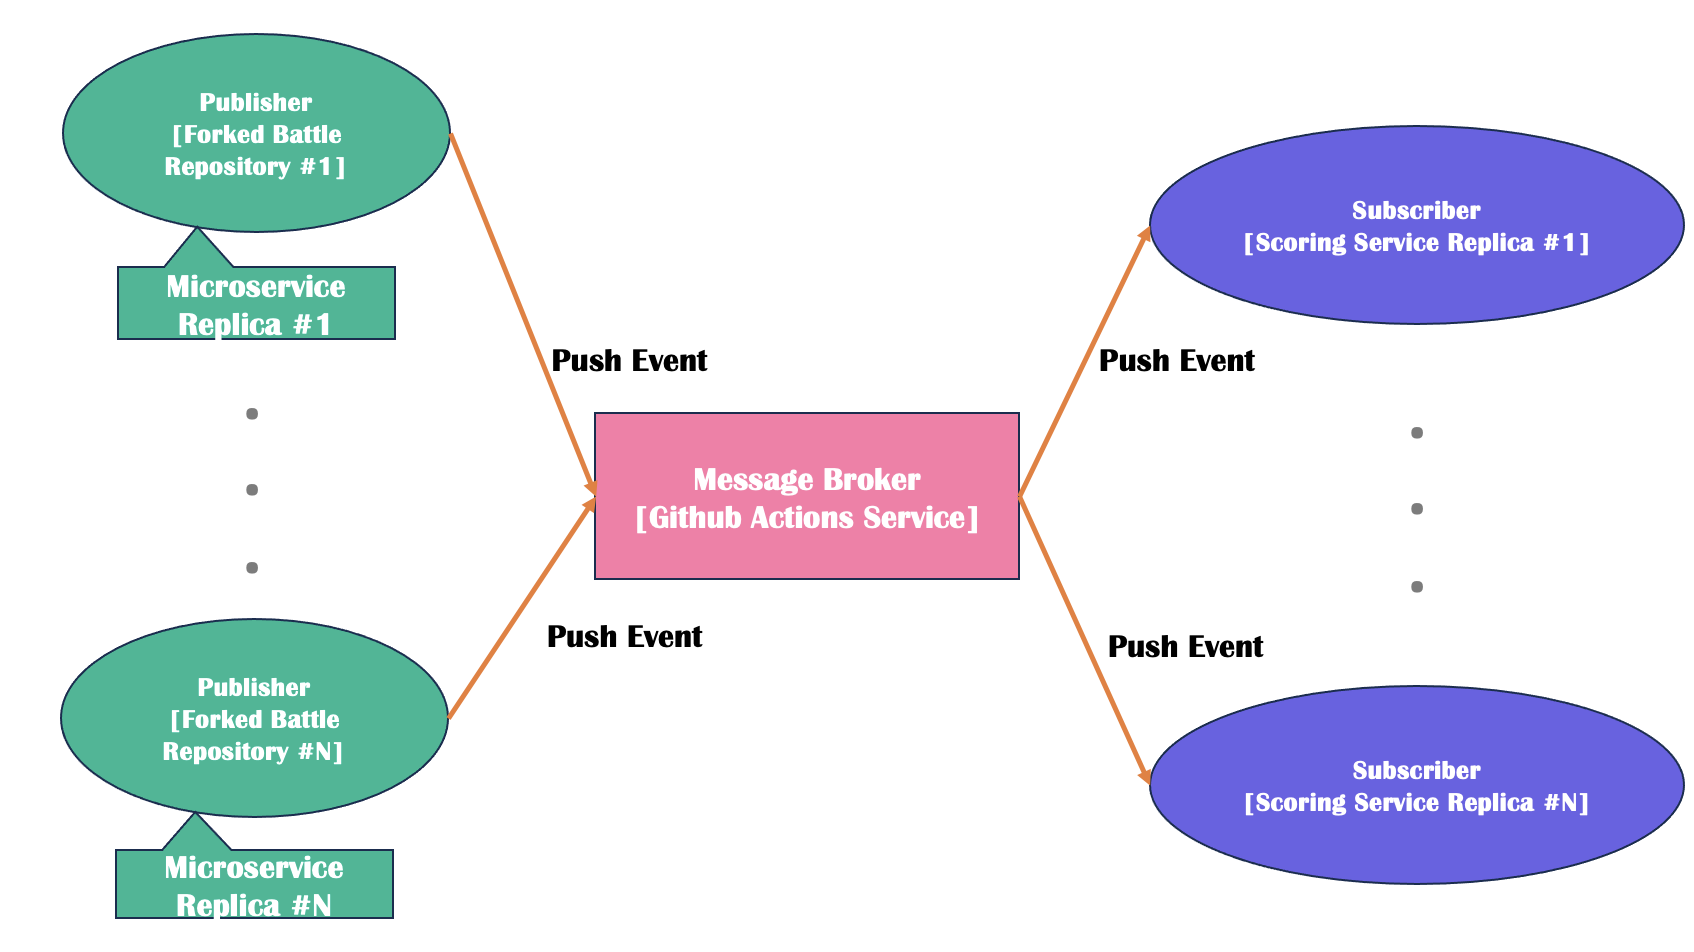
\includegraphics[width=\textwidth]{Graphics/Architecture/EventFlow.png}
    \caption{Event-driven architecture (Sub/Pub)}
    \label{fig:EventFlow}
\end{figure}


\begin{figure}[H]
    \centering
    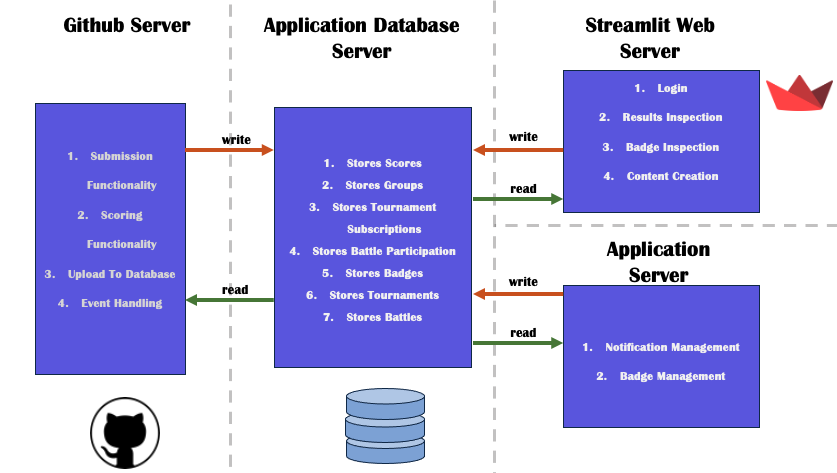
\includegraphics[width=\textwidth]{Graphics/Architecture/Physical Partitions.png}
    \caption{Physical Infrastructure Partitions}
    \label{fig:physicalpartitions}
\end{figure}


\subsection{Component view}
The components are organized into the following modules: \bigskip  \newline \textbf{User Interface Components}: \newline
 Responsible for rendering the web pages, handling user interactions, and making requests to the back-end. Individual components include:
\begin{itemize}
    \item \textbf{Front-end Service} \newline
    Represents the front-end of the application, handling user interactions, displaying information, and communicating with back-end services.
    \item \textbf{User Profile Service} \newline
    Manages user profiles, including the display of badges, tournament ranks, and overall performance visualisation
    \item \textbf{Educator Tools Service} \newline
    Provides tools and interfaces specifically for educators to create and manage tournaments, battles, and perform manual evaluations.
    \item \textbf{Authentication Service}
         \newline Responsible for user authentication and authorization.

    \item \textbf{Github Management Service}
        \newline Manages the creation and updates of relevant Github Repositories, as well as general automated communication with the Github API.
\end{itemize}
\textbf{Back-end Components}: \newline
 Responsible for processing user requests, performing application-specific functionalities and enabling the interactions between the presentation and data tier.
    \begin {itemize}
        
         %\item  \textbf{Tournament Management Service}
         %\newline Handles the creation, configuration, and management of tournaments, including setting up tournament details, deadlines, and badge criteria. It furthermore keeps track of tournament progress, participation, and tournament ranking.
         %\item  \textbf{Battle Management Service}
        %\newline Manages the creation, configuration, and deadlines of battles as well as the sign-up of participants. It triggers the creation of battle repositories through GitHub Actions, including the upload of the YAML file specific to the battle defining the submission tests customised by the educator upon battle creation. It keeps track of battle submission scores provided by the Scoring Service and updates battle rankings after each Git push.
        \item \textbf{Scoring Service}
         \newline Reads code submission test results from the database (written their by GitHub Actions) to calculate the teams battle score based on aspects such as number of tests passed, timeliness of submission and code quality levels.
        \item  \textbf{Badge Management Service}
        \newline Deals with the creation, assignment rules, and management of tournament badges. Assigns badges depending on the educator's defined rules at the end of each tournament.
        \item  \textbf{Notification Service}
        \newline Handles the notification system for informing users about new tournaments, battle updates, final battle results, and tournament badge achievements.
        \item  \textbf{Data Persistence Service (DBMS)}
        \newline Manages the storage and retrieval of data related to tournaments, battles, user profiles, scores, and badges.
         
    \end{itemize}
\textbf {GitHub Integration Components}: 

\begin{itemize}
    \item \textbf{GitHub Actions}
    \newline Used to set-up the event-driven automated testing of code submissions to forked battle repositories, upon each push. It stores test results to the system's database, where they are retrieved by the Scoring Service. GitHub Actions creates battle repositories, ultimately triggered by the Front-end Service.
\end{itemize}


\begin{figure}[H]
    \centering
    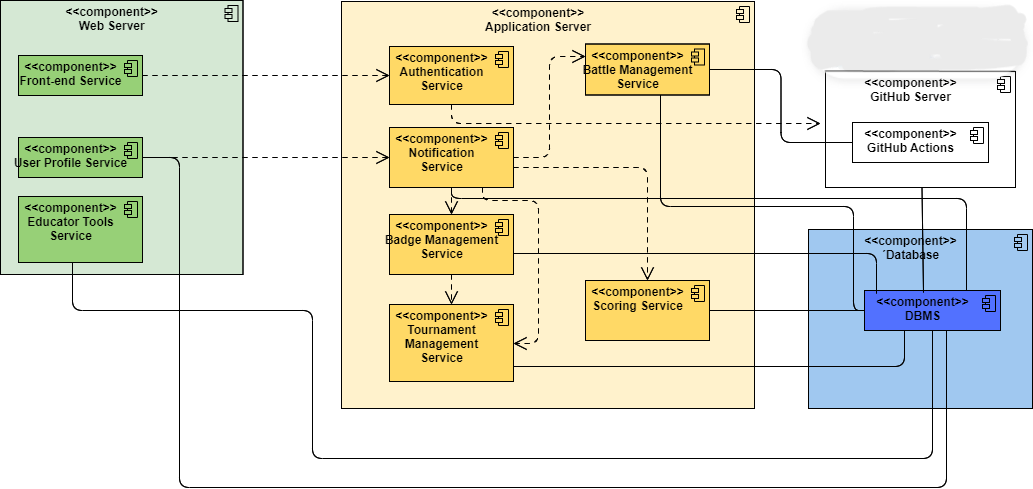
\includegraphics[width=\textwidth]{Graphics/Architecture/UML Component Diagram.png}
    \caption{Component Diagram}
    \label{fig:componentDiagram}
\end{figure}

\subsection{Deployment view}
The system will be deployed using a cloud-based infrastructure, ensuring scalability and availability. The deployment consists of:
\begin{itemize}
    \item \textbf {Web Server}: Hosts the web application accessible to users.
    \item \textbf {Application Server}: Hosts the backend modules responsible for business logic and data processing.
    \item \textbf {Database Server}: Stores user data, tournament and battle configurations, and results, as well as user data.
    \item \textbf {GitHub Actions}: Interacts with GitHub for repository hosting, version control, and automated battle code testing.
\end{itemize}
\subsection{Runtime views}
\newline
\subsubsection{Login Sequence}
\begin{figure}[H]
    \centering
    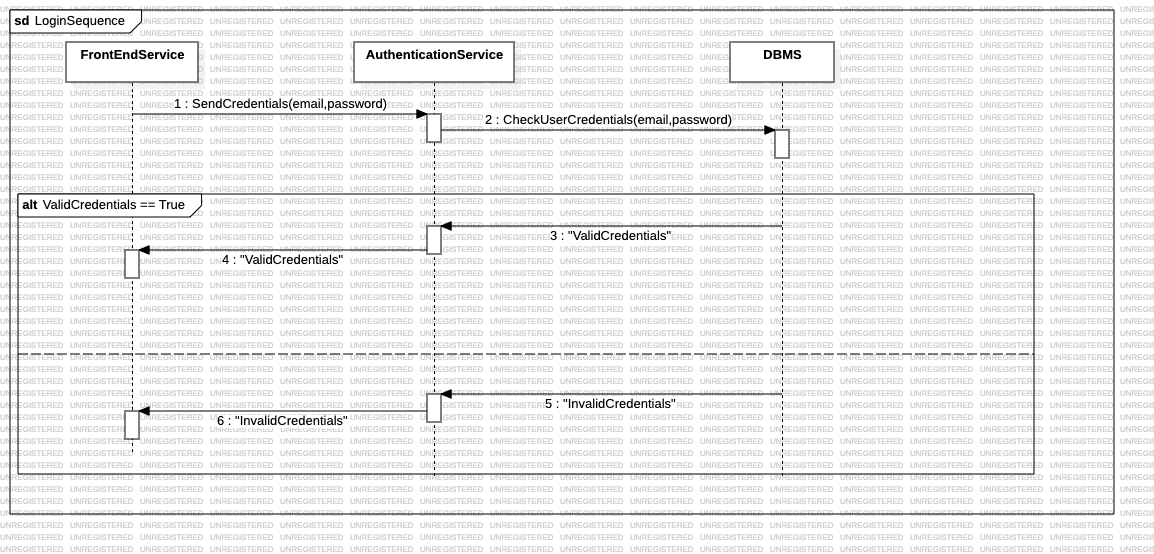
\includegraphics[width=\textwidth]{Graphics/Sequence Diagrams/LoginSequence.png}
    \caption{Login Sequence}
    \label{fig:login}
\end{figure}
The login-sequence in our case is quite simple, as the user simply inputs their credentials on the login page of the front-end. The credentials are then forwarded to the AuthenticationService which checks the validity of the credentials against the stored credentials in the DBMS. This functionality is the same, whether done as a Student User or an Educator User.

\subsubsection{Create Battle}

\begin{figure}[H]
    \centering
    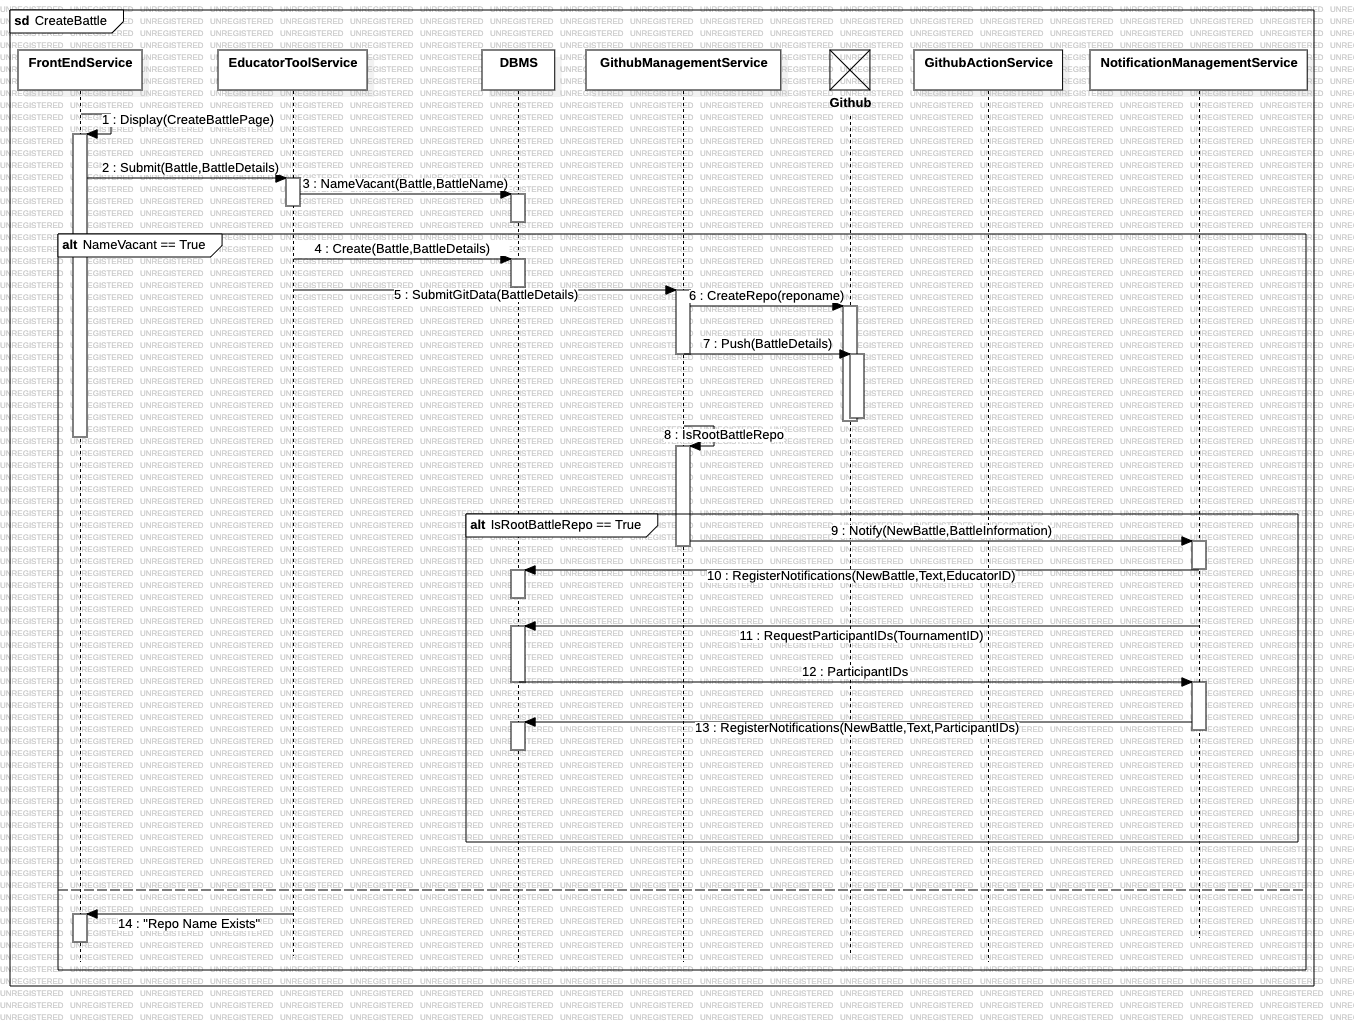
\includegraphics[width=\textwidth]{Graphics/Sequence Diagrams/CreateBattle.png}
    \caption{Create Battle}
    \label{fig:createbattle}
\end{figure}
When creating a battle in our chosen architecture, we can leverage the functionality and infrastructure of Github and Github Actions. When an Educator wishes to create a Battle, they do so through the front-end service, by simply filling in the battle details, such a name, sign-up deadline, submission deadline and description. Additionally, the Educator submits a series of test files that can be used to evaluate the submissions. When the Educator finalizes the battle creation, the front-end service first verifies that no other battle shares this name, as the name will be used in the creation of the battle's Github repository, which must be unique. If the name is unique, the Educator Tool Services can generate a repository name for the battle and officially create the Battle in the Database Management System. However, this only officially creates the Battle \textit{internally}, so a Github repository is then created from a Battle template-repository complete with Github Action YAML-files, relevant directories and so on through the Github Management Service. Subsequently, the relevant files and information from the Educator is pushed to the copied template. A check is performed to verify that this is, in fact, the root Battle repository, and not a forked submission repository. When this is verified, an action can activate the notification procedure using the Notification Management Service. The Notification Management Service first requests all userIDs of Students subscribed to the Tournament, to which this Battle belongs. Then Notifications of a new Battle is sent to all these users' email addresses.  


\subsubsection{Create Tournament}

\begin{figure}[H]
    \centering
    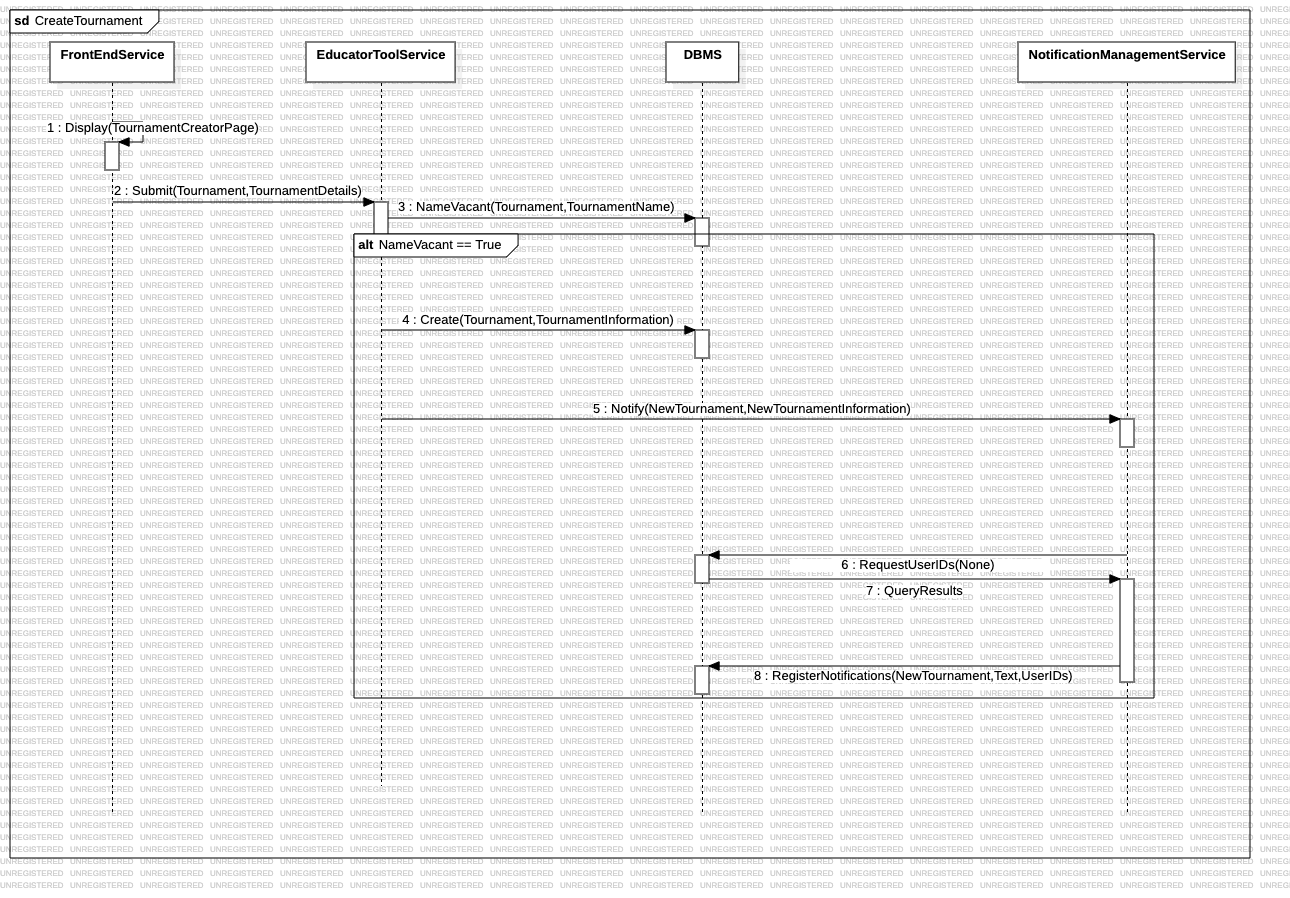
\includegraphics[width=\textwidth]{Graphics/Sequence Diagrams/CreateTournament.png}
    \caption{Create Tournament}
    \label{fig:createtournament}
\end{figure}
Creating a Tournament is much simpler than creating a Battle, as no repositories are involved yet. When an Educator creates a Tournament by filling out the CreateTournament-form through the Front-end service, the Tournament details are forwarded to the Educator Tool Service. This, in turn, checks whether the a Tournament of this name already exists. If not, the Educator Tool Service can officially create the Tournament in the DBMS. When the Front-end service refreshes, it will pick up the new Tournament from the DBMS.
Subsequently, a trigger with the relevant Tournament information is forwarded to the NotificationManagementService, which will notify all users on the platform that a new Tournament is available. 

\subsubsection{Create Badge}

\begin{figure}[H]
    \centering
    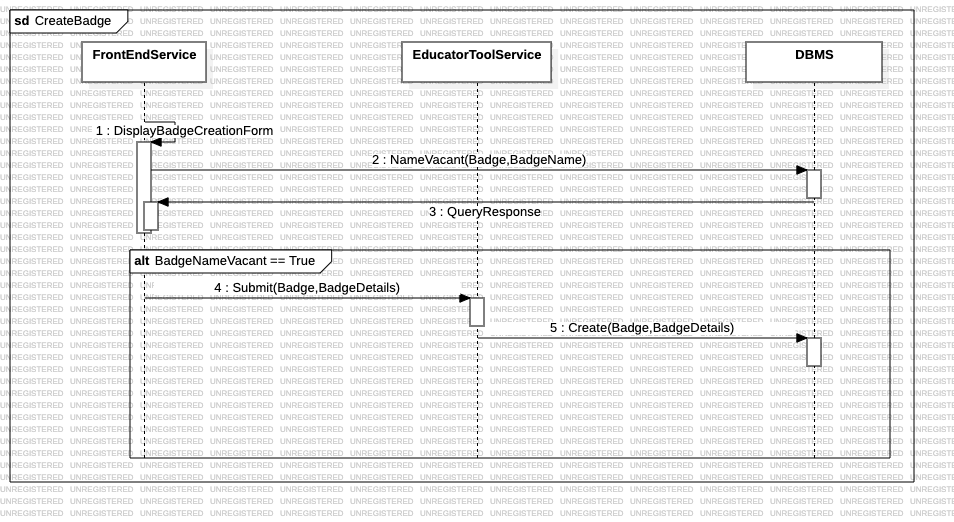
\includegraphics[width=\textwidth]{Graphics/Sequence Diagrams/CreateBadge.png}
    \caption{Create Badge}
    \label{fig:createbadge}
\end{figure}
When creating a Badge, the Educator uses the BadgeCreationForm from the FrontEndService. This form consists of a crude graphical user interface, that translates well into SQL queries. First, the Front-end Service ensures, that the badge name is unique to this tournament. If this is the case, the SQL-adjacent logic is forwarded to the Educator Tool service, and stored in the DBMS. 

\subsubsection{Receive Badge}
\begin{figure}[H]
    \centering
    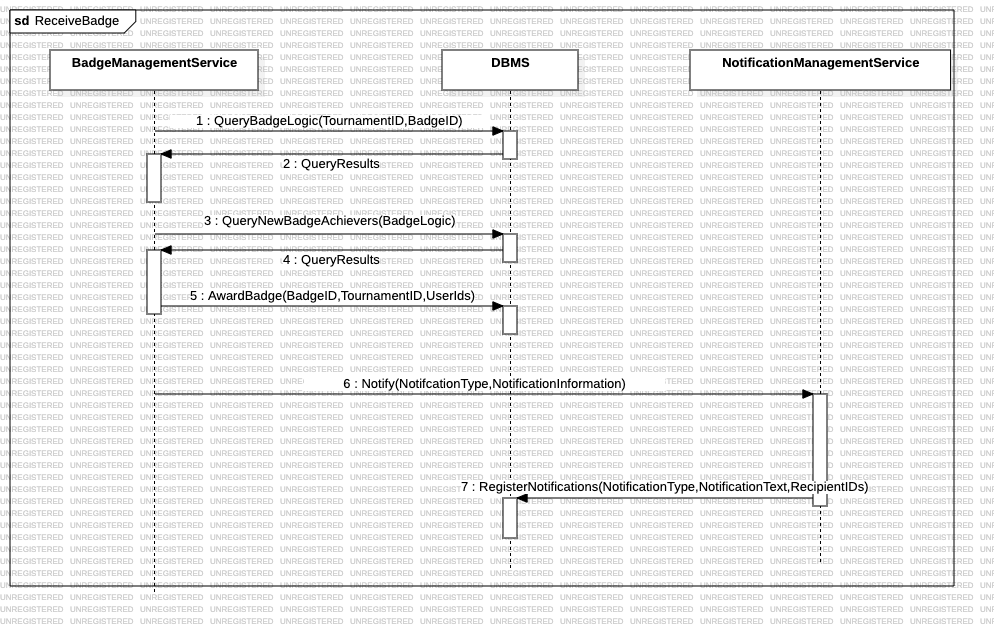
\includegraphics[width=\textwidth]{Graphics/Sequence Diagrams/ReceiveBadge.png}
    \caption{Receive Badge}
    \label{fig:receivebadge}
\end{figure}
There can potentially be quite a lot of variety in the events that can trigger a Badge. Therefore, the Badge management service simply performs a query each day, using the SQL-adjacent logic of the Badges, to retrieve all Students for all Tournaments that correspond to the queries, but have not been assigned the Badge. This solution, however, might scale poorly, as Tournaments may be active for years.

\subsubsection{Submit Solution}
\begin{figure}[H]
    \centering
    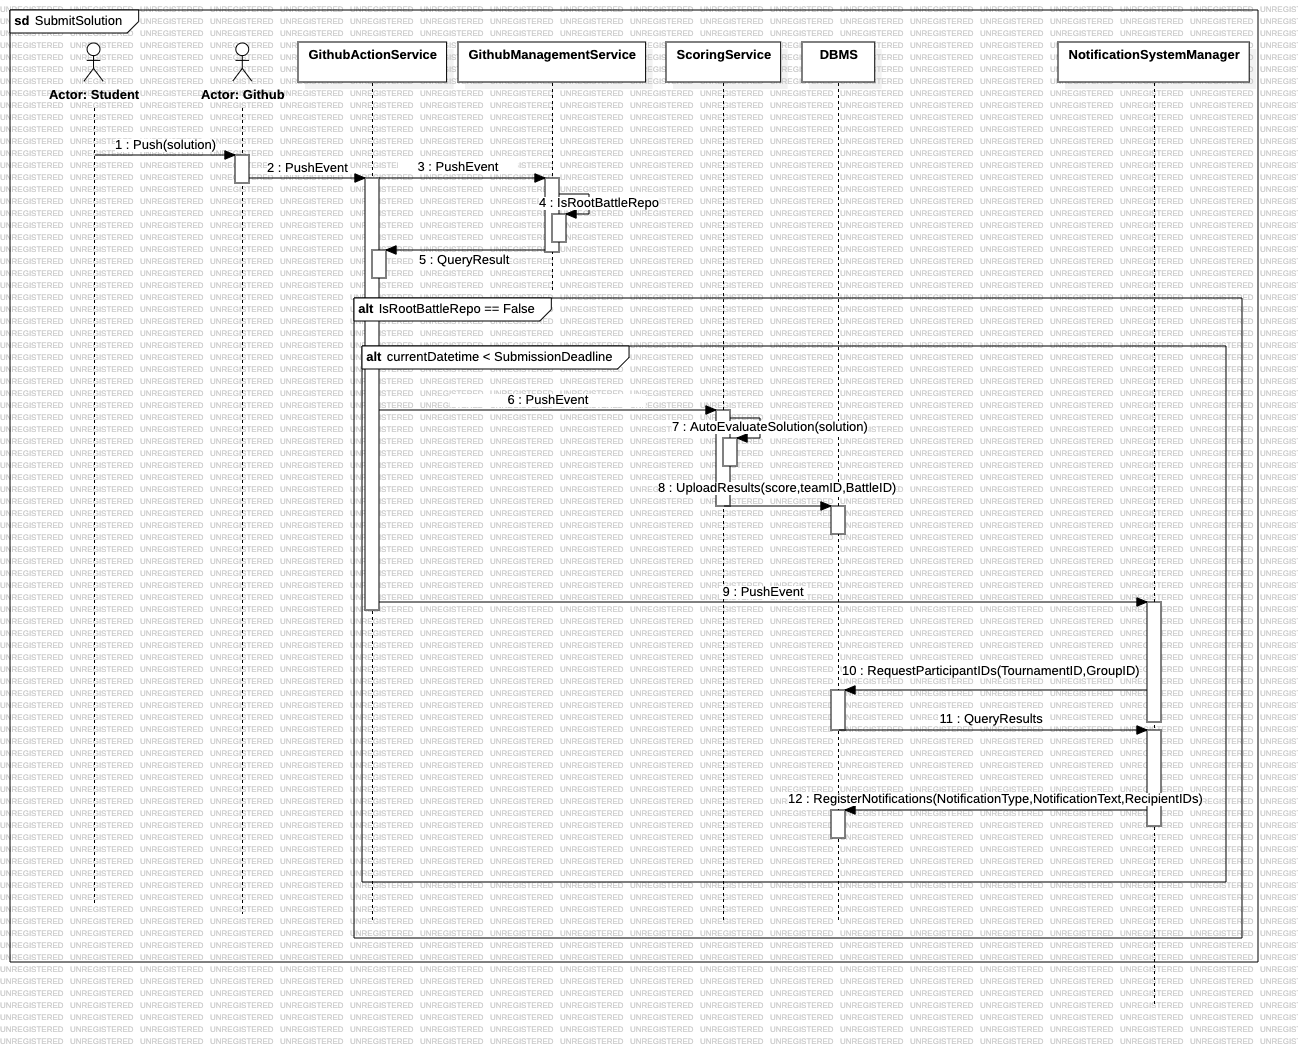
\includegraphics[width=\textwidth]{Graphics/Sequence Diagrams/SubmitSolution.png}
    \caption{Submit Solution}
    \label{fig:submitsolution}
\end{figure}
When making a Submission, we get to leverage the choice of architecture once more. When a Student performs a push to their forked Battle repository, before the deadline, it triggers the Github Action Service. The Github Action Service will follow the instructions in the Github Actions YAML-file and activate the Scoring service, automatically evaluating the Submission. The evaluation is then written to the DBMS. 
Subsequently, the YAML-file dictates that a Notification is sent to the users of the responsible group, by gathering the relevant userIDs from the DBMS.  

\subsubsection{Join Battle}
\begin{figure}[H]
    \centering
    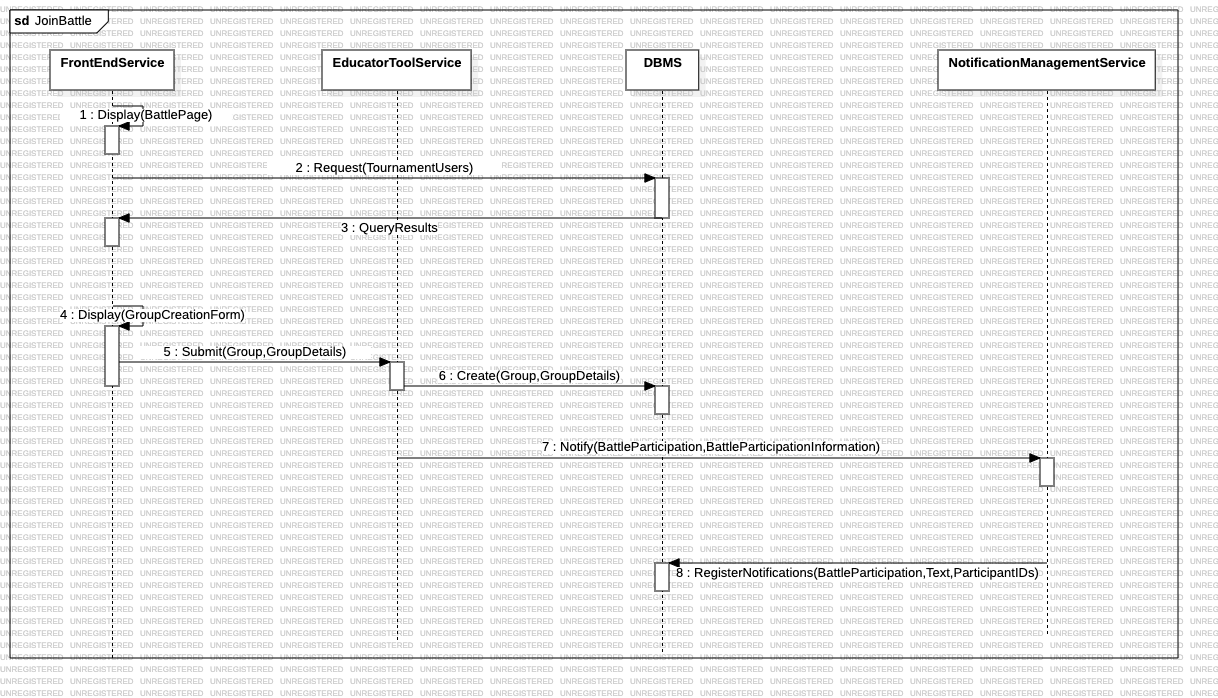
\includegraphics[width=\textwidth]{Graphics/Sequence Diagrams/JoinBattle.png}
    \caption{Join Battle}
    \label{fig:joinbattle}
\end{figure}
When joining a Battle from the Front End Service, a Student will be prompted with a drop down of the Students subscribed to the current Tournament without a group all retrieved from the DBMS. They can then select their preferred team mates, as long as they don't exceed the Educator determined threshold for group size.  The group is then written to the DBMS, through the Educator Tool Service, which manages all user-facing \textit{writes} to the DBMS, thus finalizing the group creation. The Notification Management Service is then triggered and notifies the users of their successful group formation, and Battle sign-up. 

\subsubsection{Manual Scoring}
\begin{figure}[H]
    \centering
    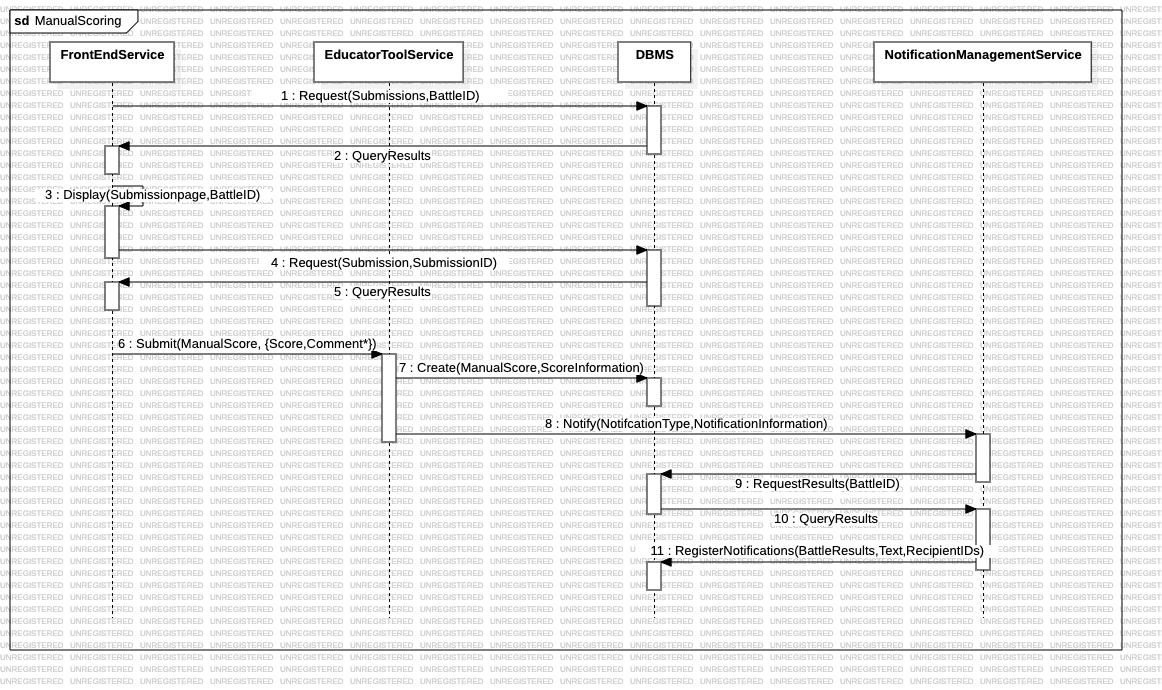
\includegraphics[width=\textwidth]{Graphics/Sequence Diagrams/ManualScoring.png}
    \caption{Manual Scoring}
    \label{fig:manualscoring}
\end{figure}
When a Battle has ended the Educator is able to assign a manual score, as well as a manual feedback to the Students. This is done throug the Front-end Service, which displays the Submissions from each Group which has received the maximum automated score. The Educator can then assign a score on the same range as the automated score, as well as a comment on the overall quality of the submission. This information is then written to the DBMS, and then notified to the responsible group through the Notification Management Service. 
The new scores will be available through the Front-end Service upon refresh. 


\subsubsection{Subscribe to Tournament}
\begin{figure}[H]
    \centering
    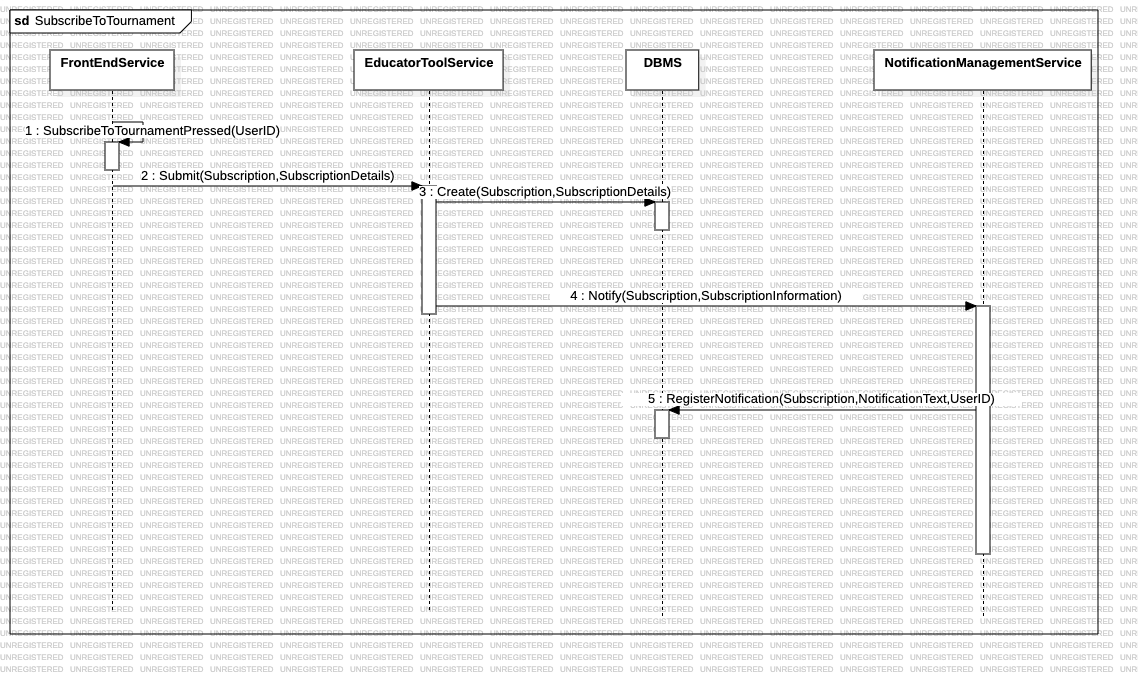
\includegraphics[width=\textwidth]{Graphics/Sequence Diagrams/SubscribeToTournament.png}
    \caption{Subscribe To Tournament}
    \label{fig:SubscribeToTournament}
\end{figure}
When a Student subscribes to a Tournament through the Front-end Service, their UserID is simply added to the DBMS, allowing the system to notify the Student of future Battles, as well as making them eligible to participate in these Battles. Immediately, the Front-end Service forwards the relevant information to the Notification Management Service, which in turn notifies the user of their successful subscription. 

\subsubsection{Announce Battle Results}
\begin{figure}[H]
    \centering
    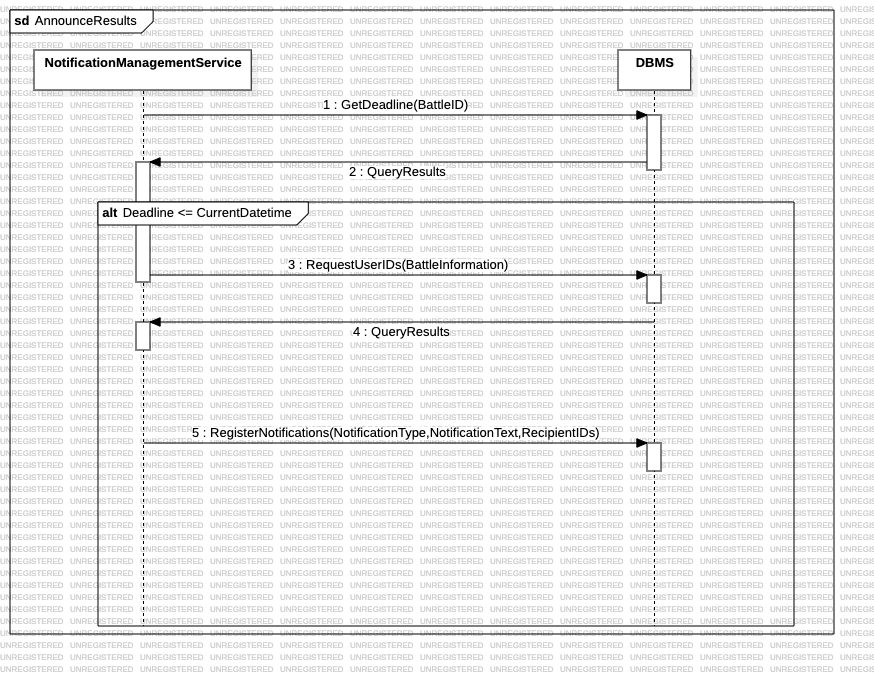
\includegraphics[width=\textwidth]{Graphics/Sequence Diagrams/AnnounceResults.png}
    \caption{Announce Battle Results}
    \label{fig:announceresults}
\end{figure}
Every day, the Notification Management Service, checks which Battles have ended since yesterday, by checking the DBMS. All participants of the Battle is then notified of their final ranking, which can also be found on the Battle page of the Front-end Service. 


\subsection{Component interfaces}
The following section aims at providing a complete list of all the methods each component interface provides to the other components.
(note: actual method names and parameters will be different based on the implementation details, we can change them later - consider these placeholders)
\bigskip \newline 
\textbf{User Interface Components}
\begin{itemize}
    \item \textbf{Front-end Service}
        \begin{itemize}
            \item Display(PageName,PageInformation)
            \item SendCredentials(email,password)
            \item Submit(Objecttype,Objectdetails)
            \item NameVacant(ObjectType,ObjectInformation)
            \item Request(data)
        \end{itemize}
    \item \textbf{User Profile Service}
        \begin{itemize}
            \item displayUserProfile(userID)
            \item updateUserProfile(userID, newProfileData)
        \end{itemize}
    \item \textbf{Educator Tools Service}
        \begin{itemize}
            \item Create(Objecttype,Objectdetails)
            \item NameVacant(ObjectType,ObjectInformation)
            \item Notify(NotifcationType,NotificationInformation)
            \item SubmitGitData(BattleDetails)
        \end{itemize}
\end{itemize}

\textbf{Back-end modules}

\begin{itemize}
    \item \textbf{Authentication Service}
        \begin{itemize}
            \item checkUserCredentials(userName, userPassword)
        \end{itemize}
    \item \textbf{Github Management Service}
        \begin{itemize}
            \item updateParticipantList(userID, teamID)
            \item IsRootBattleRepo()
            \item CreateRepo(RepoName)
            \item Push(PushDetails)
            \item Notify(NotifcationType,NotificationInformation)
        \end{itemize}
    \item \textbf{Scoring Service}
        \begin{itemize}
            \item AutoEvaluateSolution(solution)
            \item UploadResults(score,teamID,BattleID)
        \end{itemize}
    \item \textbf{Badge Management Service}
        \begin{itemize}
            \item AwardBadge(TournamentID,BadgeID,UserIDs)
            \item QueryBadgeLogic(BadgeID)
            \item QueryBadgeAchievers(BadgeLogic)
            \item Notify(NotifcationType,NotificationInformation)
        \end{itemize}
    \item \textbf{Notification Service}
        \begin{itemize}
            \item RegisterNotification(NotificationType,NotificationText,RecipientIDs)
            \item SendNotifications(NotificationType,NotificationText,RecipientIDs)
            \item RequestUserIDs(ObjectInformation)
            \item RequestDeadline(BattleID)
            \item RequestResults(BattleID)
        \end{itemize}
\end{itemize}


\subsection{Selected architectural styles and patterns}  

\subsubsection{three-tier architecture}
The system adopts a three-tier architecture differentiating between: 
\begin{itemize}
    \item \textbf{Presentation (User interface tier)}
    \begin{itemize}
        \item \textbf{Responsibility}: The presentation tier is the topmost layer and is responsible for presenting the application's user interface and handling user interaction.
        \item \textbf{Components}: This tier includes components such as user interfaces, graphical elements, and client-side logic.
        \item \textbf{Interaction}: It interacts directly with end-users, collecting user input and displaying results.
    \end{itemize}
    \item \textbf{Application logic (Business logic tier/middle tier})
    \begin{itemize}
        \item \textbf{Responsibility}: The application tier contains the business logic or application logic that processes user requests, performs application-specific functionality, and manages the communication between the presentation and data tiers.
        \item \textbf{Components}: This tier includes server-side logic, application servers, and by extension the external GitHub Server for processing business rules and workflows.
        \item \textbf{Interaction}: It communicates with both the presentation tier, the data tier, and the external service of GitHub Actions, orchestrating the flow of data and application functionality. 
    \end{itemize}
\item \textbf{Data management (Database tier)}
    \begin{itemize}
        \item \textbf{Responsibility}: The data tier is responsible for managing and storing data. It stores and retrieves data based on requests from the application tier.
        \item \textbf{Components}: This tier includes databases, data storage systems, and any components related to data storage and retrieval.
         \item \textbf{Interaction}: It interacts with the application tier to store and retrieve data as needed.
    \end{itemize}
\end{itemize}

\subsubsection{Event-Driven Architecture}
To manage the general flow of the system an event-driven architecture is adopted. In an event-driven architecture three subsystems are considered:
\begin{itemize}
    \item \textbf{Publisher:} The individually forked Battle repositories act as the Publisher of events in this system. This means that the amount of Publishers for each Battle is equal to the number of participating teams. The forked repositories have the ability to trigger one certain event; \textbf{push}.  
    
    \item \textbf{Event Broker:} The Event Broker in our system is embodied by the Github Actions Service (GAS). When a push event occurs, GAS forwards the event to the "subscribers". 
    
    \item \textbf{Subscriber:} The Subscriber in our system is the concrete GitHub Action Replica, that runs certain code whenever an event occurs. In our case, the subscriber will check if the submission is made within the time limit, making it eligible for scoring, and if so run the scoring service. 
\end{itemize}

 
\subsection{Other design decisions}
\begin{itemize}
    \item \textbf {Web Application Development Platform}: The CodeKataBattles web application will be developed using the Streamlit platform. Streamlit provides a comprehensive set of tools, libraries, and frameworks that streamline web development, ensuring efficiency.
    \item \textbf{Scalability}: %The system is designed to scale horizontally by adding more servers to the infrastructure to handle increased user load during peak times.
    The system is designed to scale vertically by upgrading the machine the system runs on. Scaling horizontally would require implementing a load balancer, which is infeasible for this minimum viable product, but the best approach when further scaling the platform. 
    \item \textbf{Security}: HTTPS is enforced for secure communication, and user authentication is handled using OAuth through GitHub credentials. We have decided to funnal all write functionality from the UI through a single service in the system (Educator Tool Service), in order to decrease the sources of potential SQL-injections. 
    \item \textbf{Caching}: Caching mechanisms are implemented to optimize data retrieval and enhance system performance.
\end{itemize}

 \subsubsection{Availability}
As described in the RASD document, the requirements of the availability of our system are not tremendous. This is in part due to the relatively low importance of this type of software, as compared to software handling critical infrastructure, sensitive data or life supporting systems. However, due to the chosen design of the system, most of the information related to ongoing battles, such as the Battle-tests, Submissions, Version control and so on, is all stored on Github's infrastructure. This means that, in the case of a breakdown, all Students in on going Battles, can continue their work, relatively unaffected, and simply receive their evaluations when the service returns. All submissions are timestamped in Github's systems, so all submissions made before the deadline will still be regarded, even if the deadline has been passed during an outage. 

 \subsubsection{Data Storage}
This architectural design aims to provide a scalable, secure, and maintainable platform for CodeKataBattles, aligning with the specified requirements.